\section{Turing-Completeness of a Language}
\label{sec:Turing Completeness}
In the dawn of computer science there were serveral ideas what computable 
means. Does it mean, that a machine can compute it, as Turing suggested? Or 
should we define some functions that should be computable and how they can be
combined to discuss the computability of a problem?

As it turned out, it does not matter -- the problems that can be solved in 
each of them are the same. This was shown by proving that the different 
mechanisms can simulate each other. By extension, a new formulism only needs 
to be able to simulate any of the existing formalisms to be at least as 
powerful as any of them. Thus came the expression {\em Turing complete} to 
describe, that a certain formalism can build any Turing machine.

This chapter is build as exercises, because solving the problems gives a good 
impression, how one could go about proving other things to be turing complete.

\subsection{The Turing Machine}
The Turing Machine (\TM) is a formalism that focuses on a possible physical 
implementation of a computing machine, although far from what is used today. 
It features an potentially infinite amount of tape on which the machine 
operates. From this tape, the machine can read and write the current cell and 
move its read-write-head one cell to the left or the right. Finally, the 
machine has a finite number of ``states of mind", comparable to a finite 
state machine.

In order to formally analyse the \TM, we can code what such a machine would 
do in the following way:

\begin{defn}
	\label{def:tm}
	A Turing Machine is a \TODO
\end{defn}

\begin{example}
	Adding one to a binary number. \TODO
\end{example}

\subsection{\WHILE is Turing complete}
By definition~\ref{def:power}, we would need a compiler from \TM to \WHILE, 
but by~\ref{thm:power-interpreter}, an interpreter suffices. Implementing such an 
interpreter will be the following exercise.

\begin{Exercise}[title={Interpreter for \TM},label={exc:tm},difficulty=2]
	\Question Show that we can implement a dictionary datastructure in \WHILE\@.
		Implement {\tt insert} and {\tt lookup}.
	\Question Show how you can code the transition function in your map.
	\Question Implement the tape
		\subQuestion Can you keep track of your position in a list with two stacks?
		\subQuestion Implement the left and right movement 
		$\interpret{{\tt left}},\interpret{{\tt right}} : Tape \rightarrow Tape$. Note that the list is 
			only potentially infinite, so you might in actuality run into the current edge.
	\Question Plug the pieces together to implement an interpreter {\tt turing(TM)} for turing machines.
		\subQuestion How many nested {\tt while} loops do you need?
\end{Exercise}
\begin{Answer}
	\Question Since execution time is not an issue, we can implement this as a 
	list of pairs:

\begin{verbatim}
    lookup read (Table.Key) {
      FOR (K.Value) IN Table {
        if [and](K = Key . [not](Result)) {
          Result := Value
        }
      }
    } Write Result

    insert read (Table.(Key.Value)) {
      Outtable := Nil
      FOR (K.V) IN Table {
        if K = Key {
          Outtable := cons (Key.Value) Outtable
        }
        else {
          Outtable := cons (K.V) Outtable
        }
      }
    } write Outtable
\end{verbatim}

If you wanted to get rid of the copying of the whole list, you could also 
just prepend the new pair, since the lookup takes the first match.
	\Question The transition function 
	$\delta: TapeAlphabet \times State \rightarrow TapeAlphabet \times State\times \{L,N,R\}$
	can be coded by taking the alphabet and the states as symbols (or numbers) 
	and storing {\tt ((in-letter.in-state).(out-letter.out-state.direction))} 
	in the map {\tt M}. Now $\delta = \interpret{spec}(lookup.M)$.
	\Question
		\subQuestion We can do that by keeping one stack {\tt left} and one for 
		{\tt right}, the idea being, that the top of the {\tt left} stack is the 
		cell adjacent to the current to the left and the top of {\tt right} is 
		the same to the right. $Tape$ could now look like {\tt (left.current.right)}
		\subQuestion 
\begin{verbatim}
  left read (left.current.right) {
    right := cons current right
    if left {
      current := hd left
      left := tl left
    }
    else {
      current := :blank
    }
  } write (left.current.right)
\end{verbatim}
and analogously for {\tt right}.
	\Question
\begin{verbatim}
  TM-step read (state.(left.current.right).transition-map)) {
    (state.current.dir) := [lookup](transition-map.(state.current))

    if (dir = :left) {
      (left.current.right) := [left](left.current.right)
    }
    if (dir = :right) {
      (left.current.right) := [right](left.current.right)
    }
  } write (state.(left.current.right))

  TM-run read (start-state.tape.transition-map.end-states) {
    current-state := start-state
    while [not]([contains](end-states.current-state)) {
      (current-state.tape) := [TM-step](current-state.tape.transition-map)
    }
  } write (current-state.tape)
\end{verbatim}
	This needs just the main loop.
\end{Answer}

\subsubsection{\TM  is \WHILE-complete}
It could now be, that \WHILE is more powerful than \TM, so that one can 
actually compute more with a \WHILE program than one could with Turing 
Machines alone.

\begin{Exercise}[title={Interpreter for \WHILE in \TM},difficulty=4]
	In this exercise, we will build up a language that can be expressed in \TM 
	and will finally include \WHILE. This is complex, but you might solve 
	many low level implementation problems of programming languages in the progress.
	\Question Show an $n$-taped \TM to the one taped (where $n$ is of course fixed at
		compilation time). A $n$-taped turing machine has $n$ tapes that can be 
		independently moved and writen. {\em Hint: Unify the tapes and mark where 
		you are.}
	\Question Show that for all \TM's {\tt A} and {\tt B} exists a turing 
			machine {\tt A;B} such that $\interpret[\TM]{A;B}(x) \peq
			\interpret[\TM]{B}(\interpret[\TM]{A}(x))$, i.e. that you can execute
			\TM's one after another.  
	\Question Show that you can implement a {\tt while} construct
		\subQuestion Given a \TM $A$ that prints {\tt T} or {\tt F} on a tape and 
			another \TM $B$, construct a \TM {\tt if A \{B\}} that runs $A$ 
			and then $B$ only if the second tape shows $T$.
		\subQuestion Modify this so that $B$ gets executed as long as $A$ returns {\tt T}.
	\Question Implement the {\tt cons} datastructure on the tape of a turing 
	machine. Note that you can add another tape to ``take notes" by merit of the first question.
		\subQuestion Implement {\tt cons}. {\em Hint: Be literal about 
		expressions like {\tt cons (cons nil nil) (cons nil nil)}.} 
		\subQuestion Implement {\tt hd} and {\tt tl}.
	\Question Show that you can implement a map, that can be used to save the variables.
		\subQuestion Implement a list of pairs.
		\subQuestion Given a name on one tape, can you look up the pair in the 
			list of tuples on a second tape that contains this name as the first
			component?
		\subQuestion Implement changing the variables by striking out the old 
			pair and appending a new one.
	\Question Argue, how you could now interpret \WHILE.
\end{Exercise}
\begin{Answer}
	\Question As we have only a limited amount of tape used, we can always move 
		to the far left side of our tape. Now imagine a memory/tape layout like 
		this (in the example for $n=2$):
		\begin{center}
			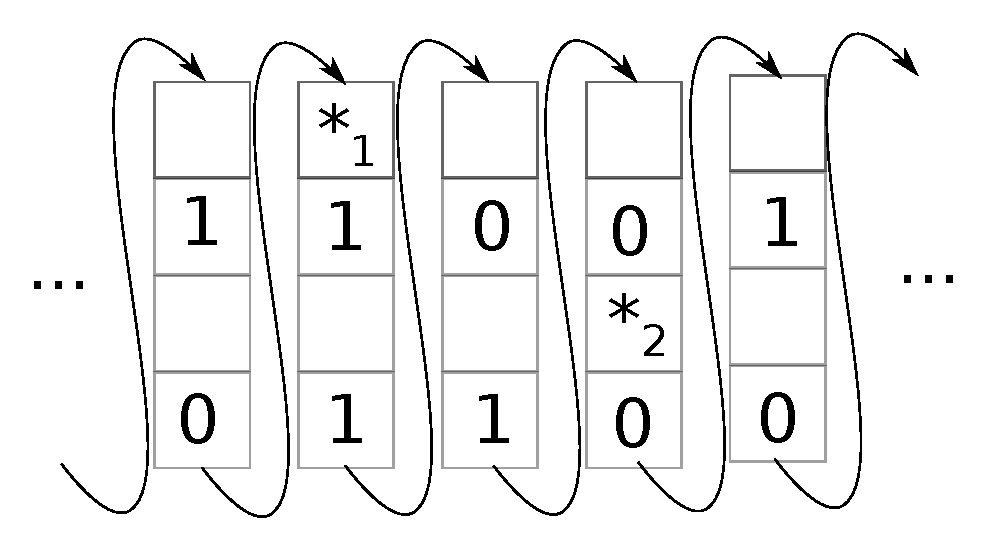
\includegraphics[width=0.49\textwidth]{computability/completeness/pictures/multitape}
		\end{center}
		where the $*_n$ means {\em tape $n$ is currently at the following value}. 
		
		Now design the states and transitions such that
		\begin{algorithmic}[1]
			\ForAll{tape $t$}
				\State move to the far left.
				\State assume state $(s, t)$, where $s$ is the state of the multi-tape machine.
				\State move right until you find $*_t$.
				\State execute the step, that the multi-tape machine would make.
				\State move $*_t$ left or right, if necessary.
			\EndFor
		\end{algorithmic}
		While this leads to a lot more states, it makes it possible to execute 
		more than one tape simultanously.
	\Question {\tt A;B} inherits the end-states of {\tt B} and the 
		starting-state of {\tt A}. The internal states of {\tt A} and {\tt B} 
		need to be disjunct, otherwise the machine could {\em jump over} from 
		{\tt A} to {\tt B} or vice versa. To ensure that, we call the states in 
		the new machine $(s, A)$ or $(s, B)$, depending on whether $s$ is from 
		{\tt A} or {\tt B}. Now $\delta((s,A), x) = \delta_A(s,x)$ and
		$\delta((s,B), x) = \delta_B(s,x)$. Finally, we connect the two machines:
		$\forall e\in Endstates_A: \delta((e, A), x) = (start_B, x, N)$
\end{Answer}

These two exercises show, that $\WHILE\epower\TM$. This is important, since 
when showing something to be \WHILE-complete, we don't need to implement the 
\WHILE, but can use \TM instead, which is much simpler.

\subsubsection{The structured program theorem}
\lineofthought{
	\begin{enumerate}
		\item run programs one after another ({\tt ;})
		\item run either this or that ({\tt if})
		\item run until predicate is false ({\tt while})
	\end{enumerate}
	$\Rightarrow$ Turing complete
}

\subsection{The Halting Problem} \label{sec:halt}
We saw in the introduction, that there are problems, that can be solved in
\WHILE, that can not be solved in \FOR and also that serveral formalisms are
equally powerful to \WHILE, so that one can wonder, if this literally solves
all problems.

Unfortunately, a simple cardinality argument shows that this is not the case: 
There are only countably infinitely many \WHILE programs, as there are only 
so many finite strings, some of which are also \WHILE programs.

The set of functions $\N \rightarrow \N$ however is bigger, as every freshmen 
course in mathematics will show.

Therefore, there must be some functions that can not be computed with \WHILE 
programs. This proof is unsatisfying, as it does not give a problem that 
can't be solved. In fact, we would again describe problems in a finite way, 
so the argument is mood.

There are however many problems that can explicitely stated but not solved by 
any algorithm. The perhaps most notoric is the halting problem:

\begin{theorem}[Halting Problem]
	There can be no program $\mathtt{halt?}\in \WHILE$ such that 
	\begin{align*}
		\interpret{\mathtt{halt?}}&:\WHILE\times \Input[\WHILE] \longrightarrow \{True, False\}\\
		\interpret{\mathtt{halt?}}&(p, i) =\begin{cases}
			False, &\text{ if }\interpret{p}(i)=\bot\\
			True, &\text{ else}
		\end{cases}
	\end{align*}
	So $\mathtt{halt?}$ answers if a given program with a certain input will halt.
\end{theorem}
\begin{proof}
	The proof is a variation of the quintessential uncomputability proof: We 
	assume that we had $\mathtt{halt?}$ and construct a program, that leads to a
	contradiction. The program is a variation of {\tt inverse}:

	\begin{verbatim}
		loopInverse read P {
		  if [halt?](P.P) {
		    while True { }
		  }
		} write P
	\end{verbatim}

	So we should get
	\begin{equation*}
	 \interpret{loopInverse}(p) = \begin{cases}
			\bot, &\text{ if }\interpret{p}(p) \neq \bot\\
			p,& \text{ else} 
		\end{cases}
	\end{equation*}
	what then is $\interpret{loopInverse}(loopInverse)$? Either it loops or it 
	returns, so lets first assume that it loops:

	\begin{align*}
		\interpret{loopInverse}(loopInverse) &= \bot &\Rightarrow \\ 
		\interpret{halt?} &= False &\Rightarrow \\ 
		\interpret{loopInverse}(loopInverse) &= loopInverse\neq \bot
	\end{align*}

	So on the other hand, what if it didn't loop?

	\begin{align*}
		\interpret{loopInverse}(loopInverse) &\neq\bot &\Rightarrow \\
		\interpret{halt?} &= True & \Rightarrow \\
		\interpret{loopInverse}(loopInverse) &= \bot
	\end{align*}

	Therefore no such \WHILE program can exist.
\end{proof}

Lets reflect on this proof: While it does use \WHILE, it would be easy to 
translate {\tt loopInverse} into other languages and give a halting 
problem for those. In fact, if we can compile {\tt loopInverse} into a 
language, then the new language can not solve its own halting problem, even 
if it was more powerful than \WHILE.

\begin{theorem}
	No language more powerful than \WHILE can solve its own halting problem.
\end{theorem}

\subsection{The Normal Form Theorem}
\begin{theorem}[Normal Form Theorem]
	Every \WHILE program can be transformed into a \WHILE program with exactly 
	one {\tt while} loop. That is, all the inner constructs are taken from \FOR.
\end{theorem}
\begin{proof}
	Lets call the language of \WHILE programs, that are in the normal form $\WHILE_1$.
	We have seen that we can transform $\WHILE \rightarrow \TM$ and 
	$\TM \rightarrow \WHILE_1$. If we chain these (informal) compilation processes to 
	get a compiler $\WHILE \rightarrow \WHILE_1$.
\end{proof}

\subsection{Church's Thesis}
As mentioned, when the notion of computability was first developed, there 
were competing formalisms, but as it turned out, they were all equally 
powerful. This lead Alonzo Church to conjegure, that what the human sees 
as intuitively computable, is adequately formalized by any of these 
competitors. This is known as Church's Thesis (or Church-Turing Thesis).

\begin{theorem}[Church's Thesis]
	The Turing Machine adequately models what we hold for intuitively computable.
\end{theorem}

We saw that \WHILE too is a competitor, since it is equally powerful to any 
of the other formalisms. We could then formulate it as follows:

\begin{theorem}
	There is no intuitive extension of \WHILE that is more powerful than \WHILE.
\end{theorem}

For example, we could add procedure calls, but that would not make any 
functions computable that were not computable before.

The thesis can not be formally proven, since it connects the informal concept 
of ``intuitively computable" with the formal Turing Machines, however the 
evidence that no-one has since build a computer, that could be exploited to
calculate more than a \TM gives a strong indication, that the Church-Turing
Thesis is true.

\subsubsection{\dots or is it?}
There has been some work, what would happen, if you added certain 
functionalities to Turing Machines (and by extension to \WHILE). 

Turing himself analysed socalled oracle machines, which are basically Turing 
Machines, but can answer specific questions to an oracle on a different tape, 
that would answer if a specific predicate is true for the value of the tape.
The halting problem for Turing Machines is not solvable on a normal \TM, but 
we could add an oracle for it. This would be more powerful than \TM, but it 
is not intuitively clear how one could build such an oracle. Also, we would 
find, that the oracle machine could not solve its own halting problem -- for 
very much the same reason that the original \TM can't solve its own.

Another line of thought is that, when we talk about these formalisms, we 
don't really care if humans find it intuitively computable, but rather that 
we could actually build a machine that computes it. This gives us the 
physical Church-Turing thesis: It is not possible to build a computer that 
can not be simulated on a \TM.

This is a thesis, that {\em can} be put to the test. While \TM rely on 
classical mechanics, some thought has been put into quantum computing. The 
model that is used to build quantum computers (qubits) are however not 
stronger than \TM. Faster yes, but not really stronger.

On a larger scale, it is possible to construct a computing device that orbits 
around a rotating black hole. An observer falling into the black hole could 
then observe the infinite computation time of the orbiting machine in
subjectively finite time\footnote{See \cite{etesi2002blackhole} for the whole
discussion on the feasability and the mathematical proof}. It has however been
noted, that falling into a black hole might not be a good idea\citationneeded.

\lineofthought{
	List some surprisingly turing complete things, e.g. cellular automata (Rule 110), 
	string rewriting, ...

	Churches thesis: There is no intuitive extension to {\tt  WHILE} that is 
	stronger than {\tt WHILE}.

	Approximations of results, ... also work (linear slow-down). 

	Note that when there are side effects, we might be interested that a program
	does {\em not} terminate (e.g. our OS).

	Common features of turing complete languages: They can use their own 
	description (recursion theorem), if there is a primrec subset $P$, then you 
	can describe all programs with $P$ and one ''loop`` of $A\setminus P$ 
	(normal form theorem)
}

\subsection{Properties of Turing complete languages}

\lineofthought{
	\begin{itemize}
		\item Recursion theorem (explain the construction of the $Y$ combinator)
		\item Normal form theorem
		\item Can't solve the halting problem
		\item Can't deduce a property of $\interpret{f}$ from $f$ alone in full generality. (Rice)
	\end{itemize}
}
\subsection{Why are most programming languages Turing Complete?} % (fold)
\label{sub:Why are most programming languages Turing Complete?}
\lineofthought{
	While most algorithms used today are guaranteed to stop, proving this for all
	programs of a language is often hard. Things like recursion is no longer
	possible, unbound conditional loops (`while`) don't work and there are real
	problems that can not be solved this way. 

	Compare however Coq, that is {\em not} Turing Complete, but still used.
}
% subsection Why are most programming languages Turing Complete? (end)
